% coding:utf-8

%----------------------------------------
%FOSADSVB, a LaTeX-Code for a summary of digital signal processing
%Copyright (C) 2015, Mario Felder & Michi Fallegger

%This program is free software; you can redistribute it and/or
%modify it under the terms of the GNU General Public License
%as published by the Free Software Foundation; either version 2
%of the License, or (at your option) any later version.

%This program is distributed in the hope that it will be useful,
%but WITHOUT ANY WARRANTY; without even the implied warranty of
%MERCHANTABILITY or FITNESS FOR A PARTICULAR PURPOSE.  See the
%GNU General Public License for more details.
%----------------------------------------

\chapter{Multirate und Filterbänke}
\section{Downsampling/Decimation}
Um ein Signal donwzusamplen, wird einfach nur jedes $D$-te Sample verwendet.
\begin{center}
	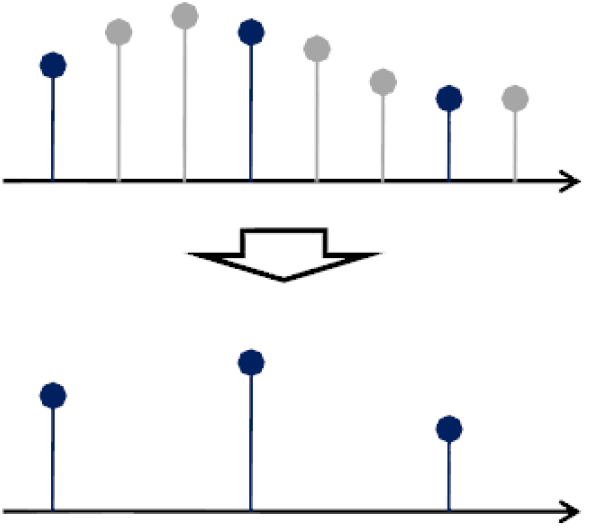
\includegraphics[width=.2\textwidth]{../fig/downsample}
	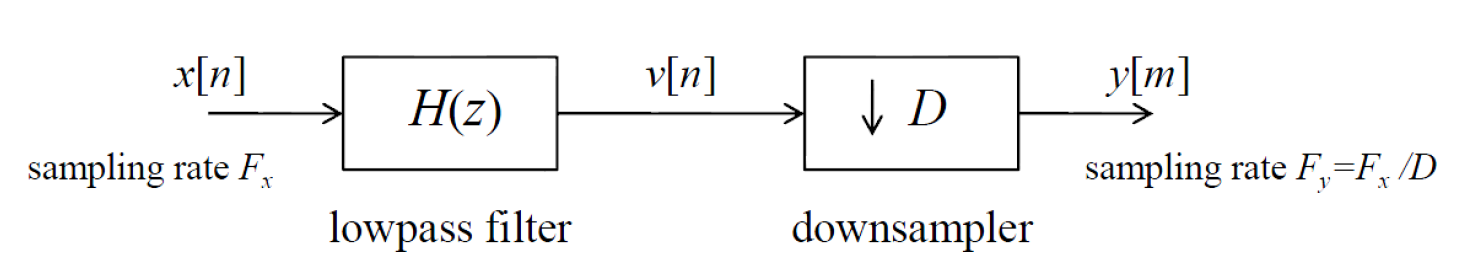
\includegraphics[width=.6\textwidth]{../fig/decimation}
\end{center}
Dabei muss beachtet werden, dass das Abtasttheorem noch eingehalten wird. Das
Signal muss zuerst mit einem Tiefpass gefiltert werden. Die Frequenzantwort des TP ist
idealerweise:
\[ H(\Omega) = \left\lbrace \begin{matrix}
	1 & \textrm{if } \Omega \in [-\pi/D,\pi/D]\\
	0 & \textrm{otherwise}
\end{matrix} \right. \] 
Das Resultat kann beschrieben werden als $y[m] = v[nD]$. Das Frequenzspektrum
wird um den Faktor $D$ horizontal gespreizt und gleichzeitig vertikal 
gestaucht. Für einen \emph{idealen} TP-Filter gilt für das resultierende Spektrum $Y(\Omega)$:
\[ Y(\Omega) = \frac{1}{D} V(\Omega/D)  \]
Allgemein für alle TP-Filter, wobei $d=1,...,D-1$ Aliasing aufgrund nicht idealer TP-Filterung einbezieht:
\[ Y(\Omega) = \frac{1}{D} \sum_{d=0}^{D-1} V(\Omega/D-2\pi d/D) \]
\begin{center}
	\includegraphics[width=.45\textwidth]{../fig/decimation_frequenz}
\end{center}
Als TP-Filter kann ein FIR Filter verwendet werden. Eine direkte Implementierung
ist nicht effektiv, da $D-1$ vom Filter berechnete Werte vom Downsampler
weggeworfen werden. Mit dem Downsampler vor dem Filter müssen weniger
Berechnungen durchgeführt werden. Die Multiplikatoren können mit einer 
tieferen Samplingrate betrieben werden. \\\\
Direkte, ineffiziente Implementation (links) \& effizientere Implementation (rechts):
\begin{center}
	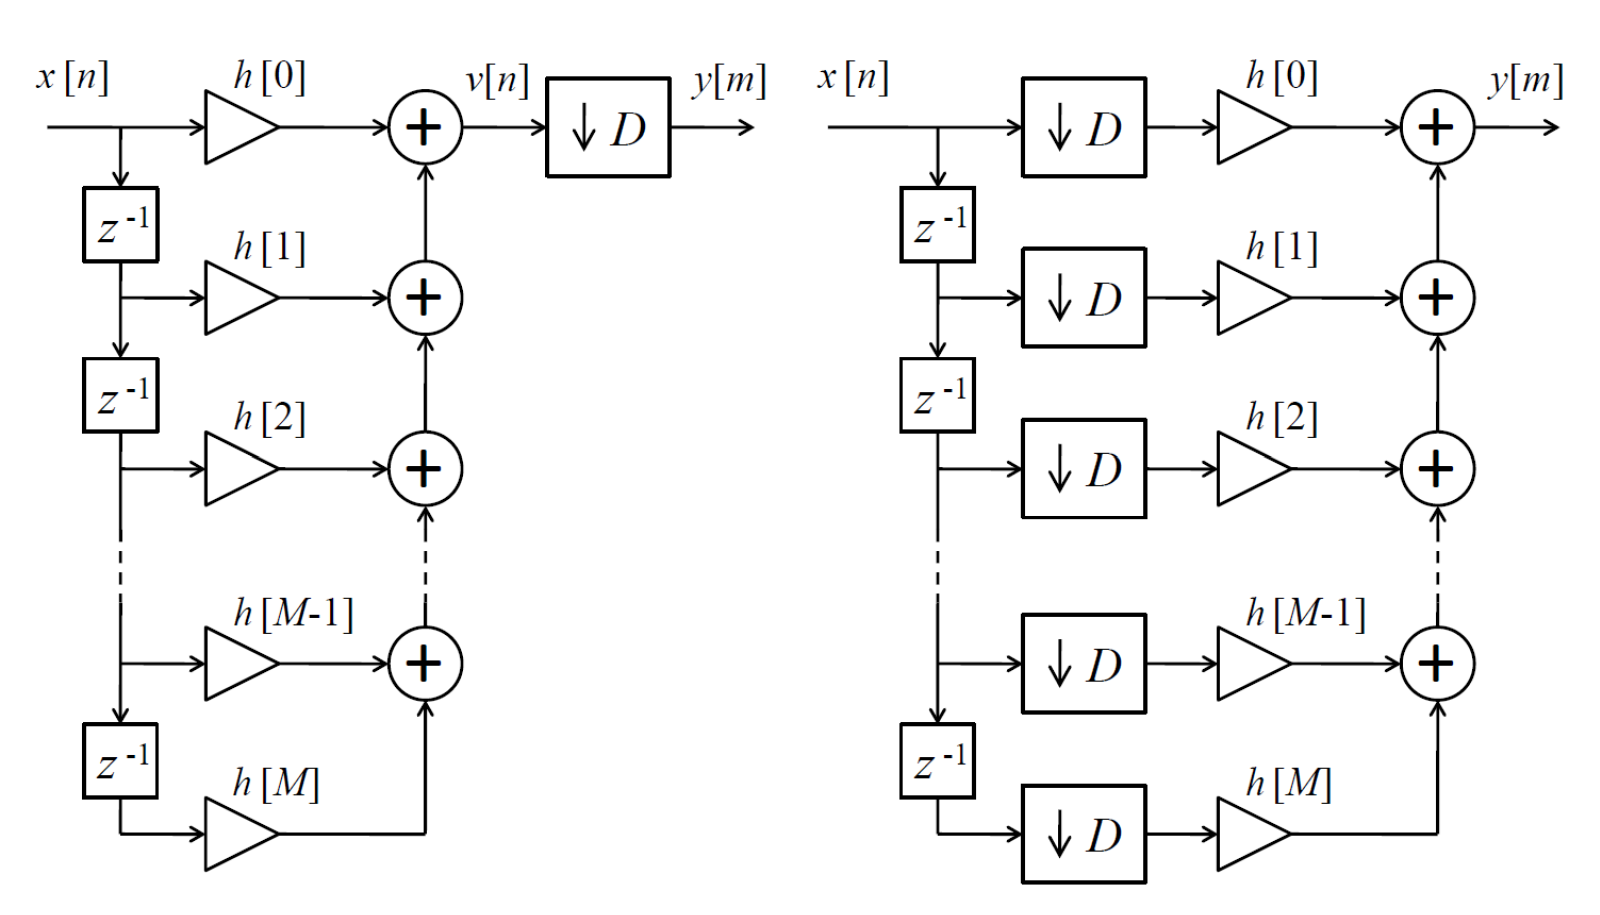
\includegraphics[width=.7\textwidth]{../fig/decimation_scheme}
\end{center}

%===============================================================================
\section{Upsampling/Interpolation}
Bei einem Upsampler mit dem Faktor $I$ werden zwischen zwei Samples jeweils
$I-1$ Nullen eingefügt.
\begin{center}
	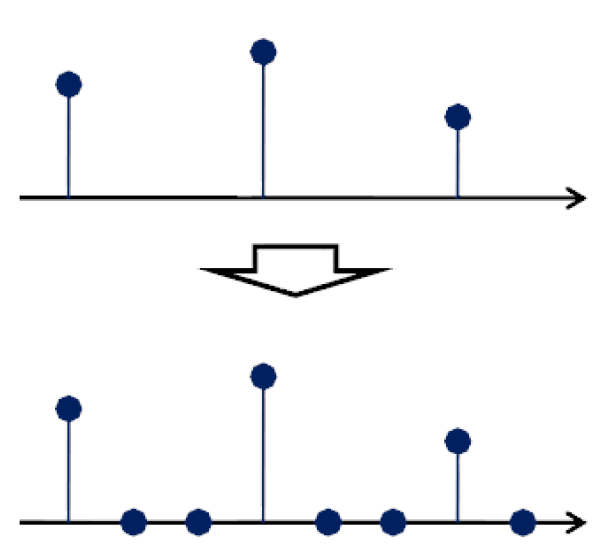
\includegraphics[width=.2\textwidth]{../fig/upsample}
	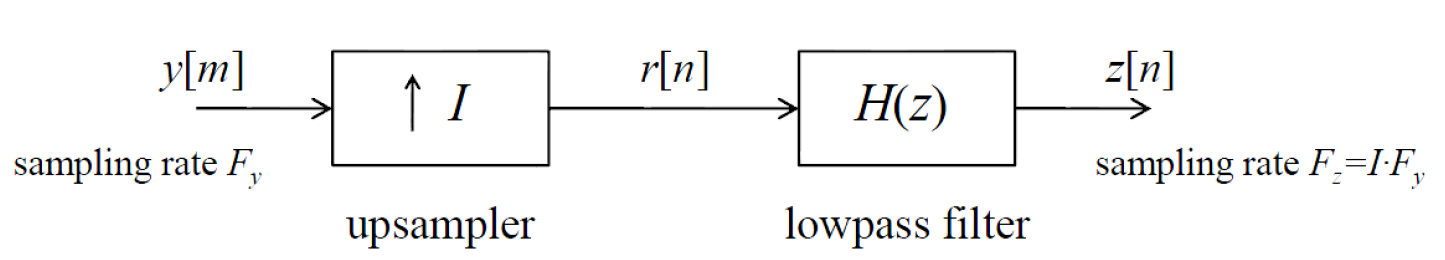
\includegraphics[width=.6\textwidth]{../fig/interpolation}
\end{center}
\[ r[n] = \left\lbrace \begin{matrix}
	y[n/I] & \textrm{if } n \in [0,\pm I, \pm 2I,\ldots]\\
	0 & \textrm{otherwise}
\end{matrix} \right. \] 
Die Abtastfrequenz $F_z$ ist $I$-mal höher als die Abtastfrequenz $F_y$ von
$y[m]$. Das Spektrum des upgesampelten Signal ist:
\[ \ R(\Omega) = \sum_{n=-\infty}^{\infty} r[n]
	\e^{-\im\Omega n} 
	= \sum_{m=-\infty}^{\infty} r[m]\e^{-\im\Omega m}
	= Y(I\Omega)  \]
Damit das Frequenzspektrum von $y[m]$ nicht periodisch mit der Periode
von $2\pi/I$ ist, ist eine Tiefpassfilterung nach dem Upsampling notwendig. 
Er glättet das Signal und führt dadurch die Interpolation durch. Der
ideale TP-Filter hat die Frequenzantwort:
\[ H(\Omega) = \left\lbrace \begin{matrix}
	I & \textrm{if } \Omega \in [-\pi/I,\pi/I]\\
	0 & \textrm{otherwise}
	\end{matrix} \right. \]

\begin{center}
	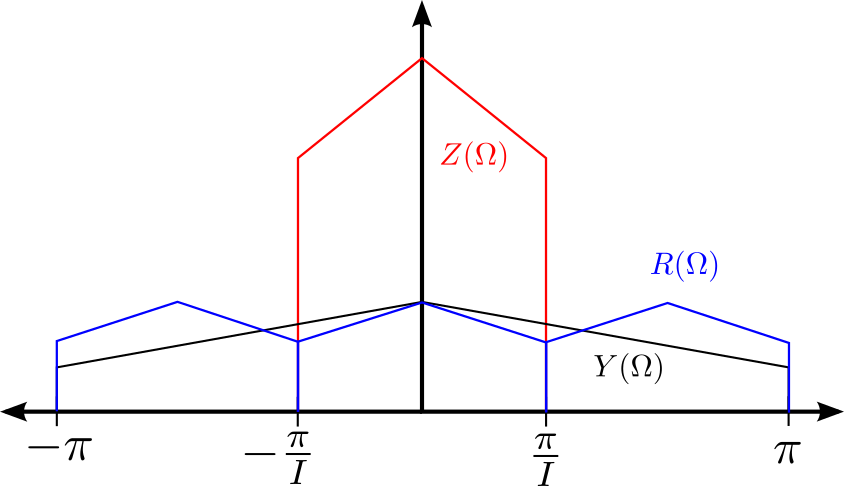
\includegraphics[width=.45\textwidth]{../fig/interpolation_frequenz.png}
\end{center}
Ein FIR oder IIR Filter kann als TP-Filter verwendet werden. Eine direkte
Implementierung (siehe linkes Blockschaltbild) ist ineffektiv, da der 
Filter auch auf die Null-Werte angewandt wird. Rechts muss der Multiplikator
nur mit der Frequenz $F_y$ arbeiten, im Vergleich zu links mit der höheren $F_z$
nach dem Upsampling.
\begin{center}
	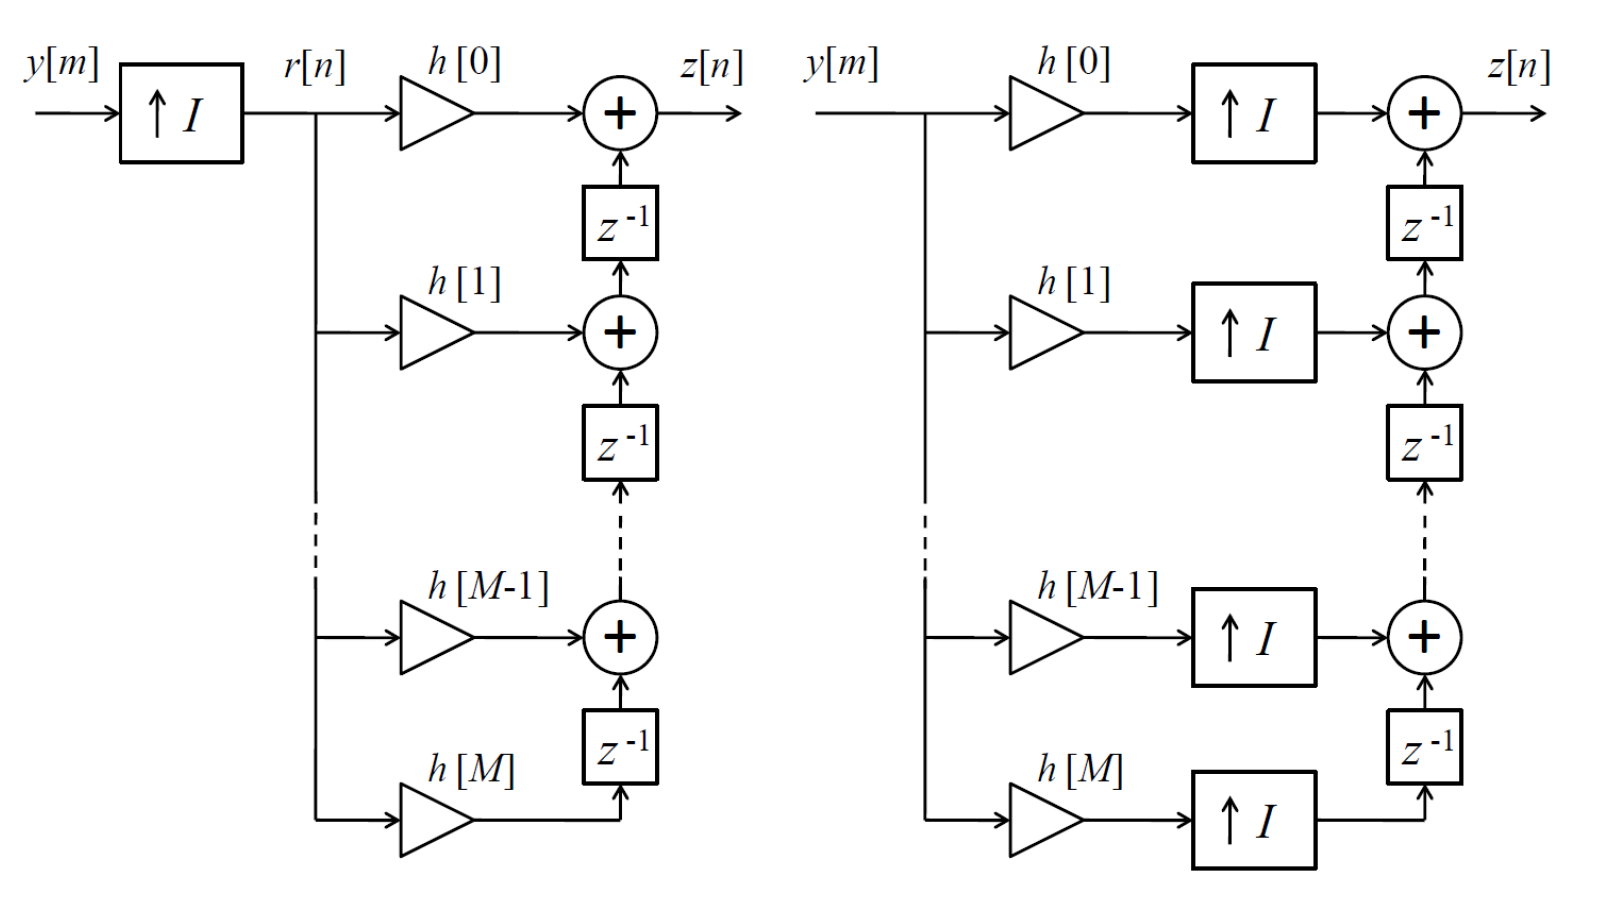
\includegraphics[width=.7\textwidth]{../fig/interpolation_scheme}
\end{center}

%===============================================================================
\section{Polyphasen Filter}
Dienen zur effizienteren Implementation von Filtern. 
Jede $i$-te Komponente von $p_i[k]$ beinhaltet den $M$-ten Koeffizienten der 
Impulsantwort $h[k]$, alle zusammen beinhalten die gesamten Informationen.
Insgesamt existieren also immer $M$ Polyphasenfilter.   
Die um $M$ downgesampelte Impulsantwort $h[k]$ ist definiert als:
\[ p_i[k] = h[kM+i] \qquad i=0,1,\ldots,M-1 \]
Dazugehörende z-Transformation für die Polyphasen-Komponenten $P_i(z)$:
\[ P_i(z) = \sum_{k=-\infty}^{\infty} p_i[k]z^{-k} \qquad i=0,1,\ldots,M-1 \]
Somit gilt für das Spektrum:
\[ H(z) = \sum_{i=0}^{M-1}z^{-i} P_i(z^M) \]
Der Vorteil liegt darin, dass die Filter bei einem Upsampling mit der Rate $F_y$ statt der höheren
Rate $F_z$ arbeiten können. Die einzelnen Werte müssen anschliessend nur noch
mit der $F_z=I \cdot F_y$ zusammengesetzt werden.\\
Bei einem Downsampling können die Filter mit $F_x/D$ arbeiten, während die Werte mit $F_x$ 
auf die einzelnen Polyphasen-Komponenten aufgeteilt werden. \\\\
\begin{minipage}{.48\textwidth}
	\centering
	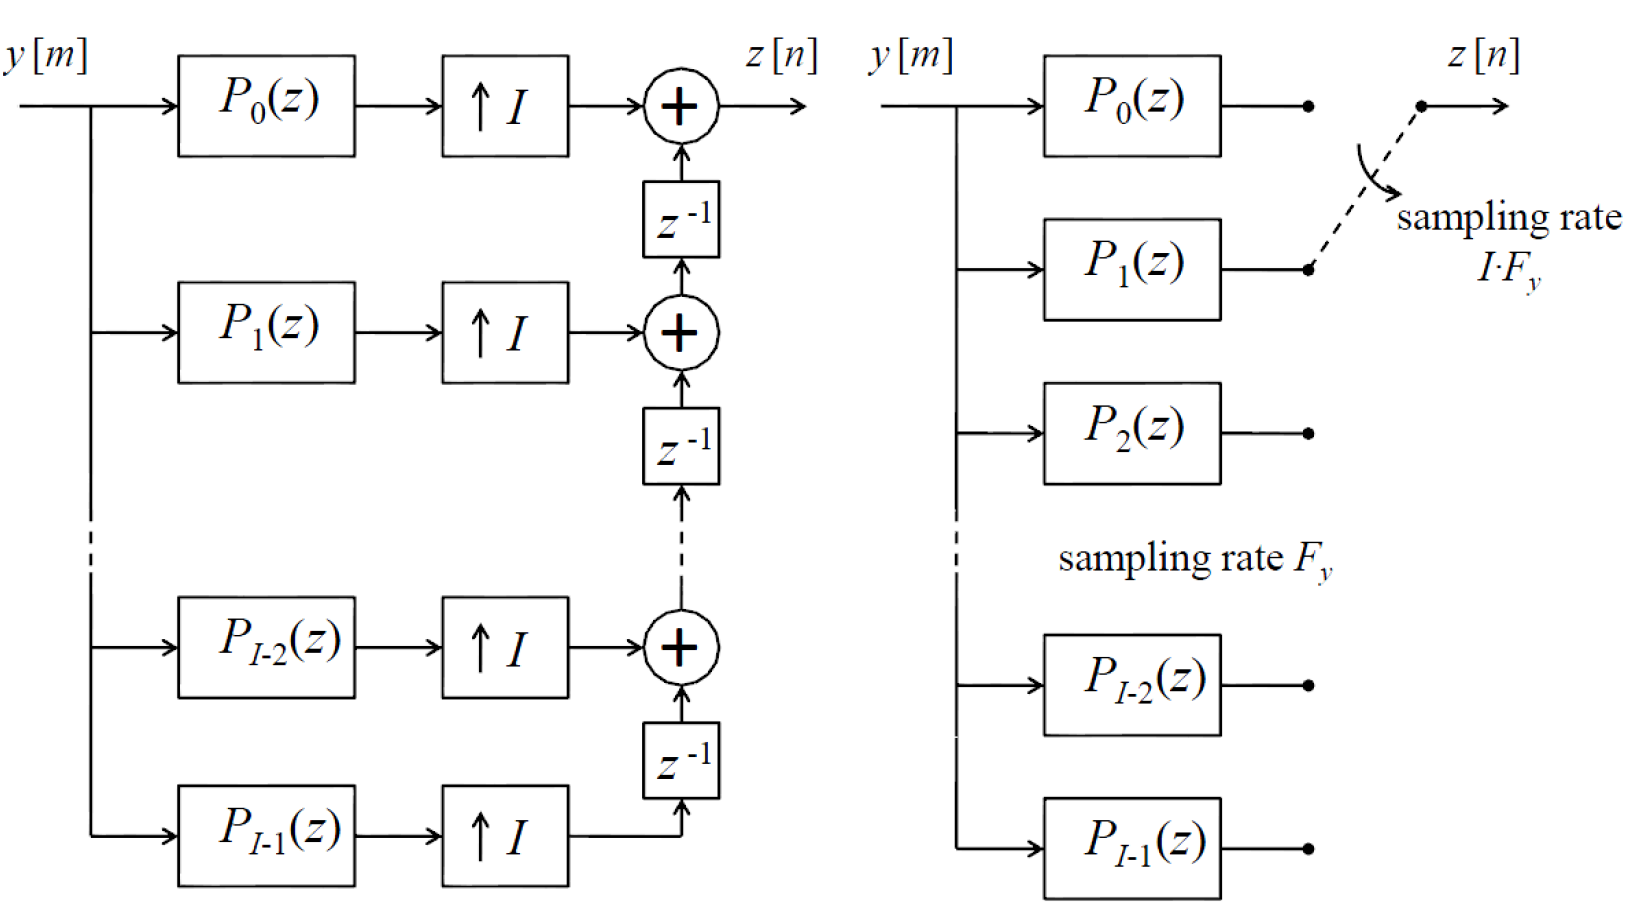
\includegraphics[width=\textwidth]{../fig/polyphase_up}
\end{minipage}
\begin{minipage}{.48\textwidth}
	\centering
	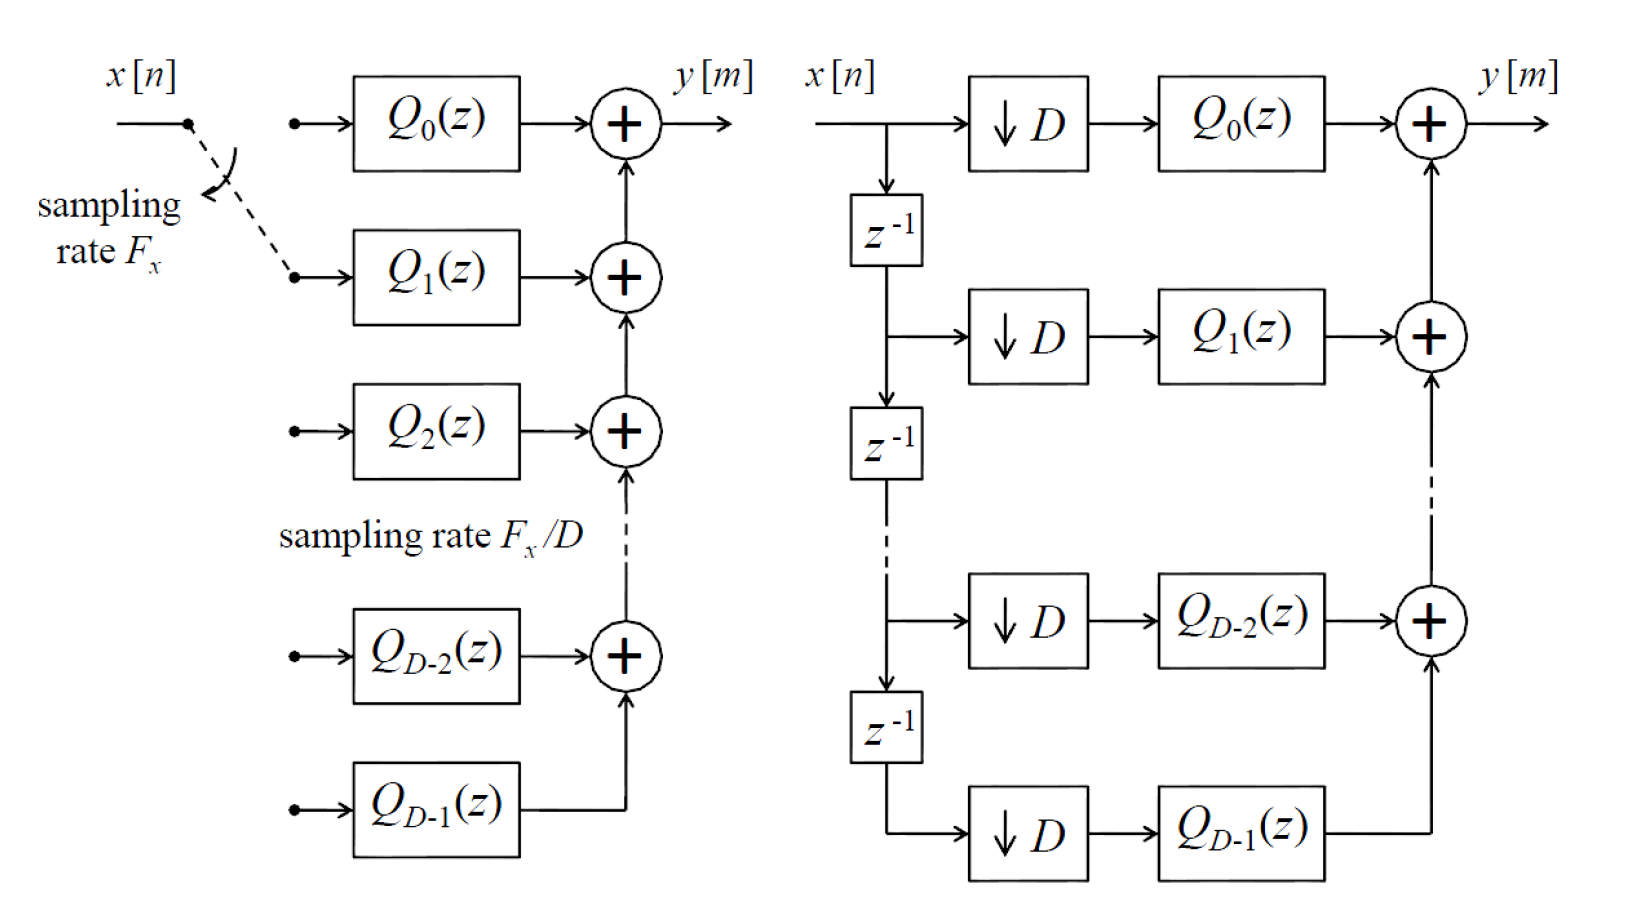
\includegraphics[width=\textwidth]{../fig/polyphase_down}
\end{minipage}
\newpage

%===============================================================================
\section{Implementation rationaler Abtastraten}
Wenn ein up- bzw. downsample Faktor gefordert ist, welcher nicht ganzzahlig ist,
kann dieser mit $\frac{I}{D}$ dargestellt werden.\\\\
Wenn zuerst der Downsampler kommt, gehen Informationen verloren. Andersrum
entsteht eine hohe Abtastfrequenz dazwischen. Es ist jedoch vorzuziehen,
zuerst das Upsampeln durchzuführen, danach das Downsamplen. So kann der Tiefpass 
der Interpolation mit dem Tiefpass der Decimation kombiniert werden.
\begin{center}
	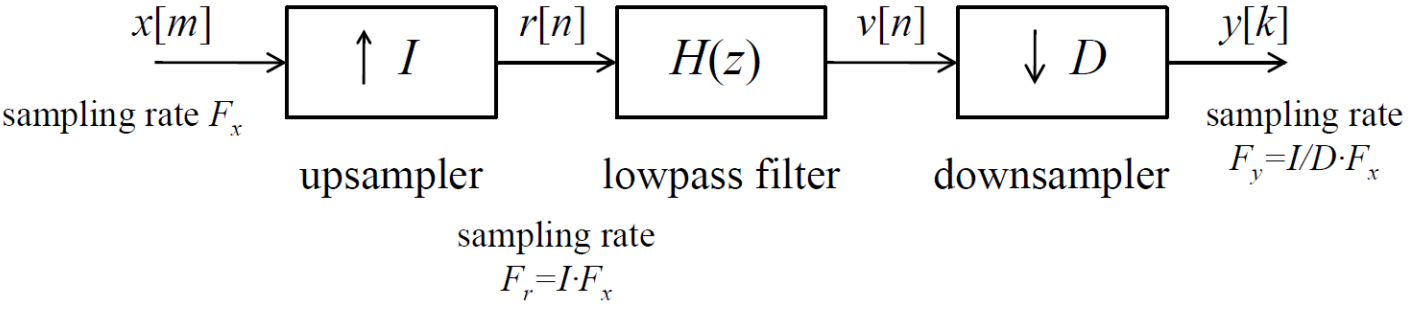
\includegraphics[width=.6\textwidth]{../fig/sampling}
\end{center}
Die Anzahl an Koeffizienten $p$ für einen FIR-TP-Filter mit Länge $N$ berechnet sich wie folgt:
\[ p = \frac{N}{I} \]
Es werden $p$ Multiplikationen sowie $p-1$ Additionen notwendig pro Output Sample des Filters.
%===============================================================================
\section{Quadratur Spiegel Filterbank}
Um den Datenverlust beim Downsampeln zu kompensieren, kann das Signal über zwei
Kanäle übertragen werden. Der eine Kanal filtert das Signal mit einem TP $H_0(z)$,
der Andere mit einem HP $H_1(z)$.
\begin{center}
	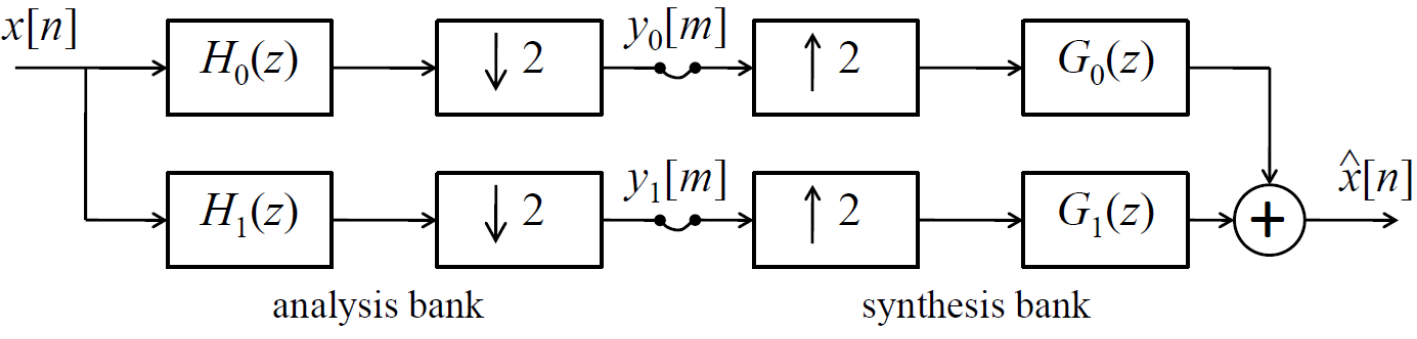
\includegraphics[width=.6\textwidth]{../fig/quadrature_mirror}
\end{center}
Die DTFT der zwei generierten Signalen $y_0[m]$ und $y_1[m]$ sind:
\[ Y_{0/1} = \frac{1}{2} \left( H_{0/1}\left( \frac{\Omega}{2} \right)
	X\left( \frac{\Omega}{2} \right) + H_{0/1}\left( \frac{\Omega}{2} - \pi
	\right) X\left( \frac{\Omega}{2} -\pi\right) \right)\]
Das Spektrum des synthetisierten Signals $\hat{x}[n]$ ist:
\[\begin{aligned} \hat{X}(\Omega) = &\frac12 \bigg( H_0(\Omega)G_0(\Omega)
	+ H_1(\Omega)G_1(\Omega) \bigg) \cdot X(\Omega) \\
	+ &\underbrace{\frac12 \bigg( H_0(\Omega-\pi)G_0(\Omega)
	+ H_1(\Omega-\pi)G_1(\Omega) \bigg) \cdot X(\Omega-\pi)}_
	{\textrm{alias term}} \end{aligned}\]
Um keinen Aliasterm zu haben müssen die Bedingungen $G_0(\Omega) = H_1(\Omega
-\pi)$ und $G_1(\Omega) = -H_0(\Omega-\pi)$ erfüllt sein.\\
Oft wird ebenfalls nur ein Filter $H(\Omega)$ gewählt. 
Meist wird dieses im $z$-Bereich bestimmt/vorgegeben und kann dann
mit $z=e^{j\cdot \Omega}$ umgewandelt werden.
Die entsprechenden Filter können dann wie folgt abgeleitet werden:
\[\begin{aligned}
	H_0(\Omega) &= H(\Omega)\\
	H_1(\Omega) &= H(\Omega-\pi)\\
	G_0(\Omega) &= H(\Omega)\\
	G_1(\Omega) &= -H(\Omega-\pi)
\end{aligned}\]
Anschliessend werden sie in den $z$-Bereich zurücktransformiert, z.B. 
$H_0(\Omega) \ \laplace \ H_0(z)$ oder $G_1(\Omega) \ \laplace \ G_1(z)$.\\
Dank dieser Transformation können die Impulsantworten einfach ermittelt werden.
\newpage \noindent
Weiter gilt für das synthetisierte Signalspektrum:
\[ \hat{X}(\Omega) = T(\Omega)X(\Omega) \qquad \text{, wobei: } 
				T(\Omega) = \frac{1}{2}\bigg(H^2(\Omega) -H^2(\Omega-\pi)\bigg) \]
Um perfekte Rekonstruktion zu haben, muss $T(\Omega)$ eine Allpass-
Charakteristik mit linearer Phasenverschiebung aufweisen (konstante Amplitudenverstärkung, konstante Zeitverzögerung). 
Dies kann am besten mit einem symmetrischen FIR-Filter (ungerade Ordnung) erreicht werden. Der einseitige Frequenzgang
sieht dann wie folgt aus:
\begin{center}
	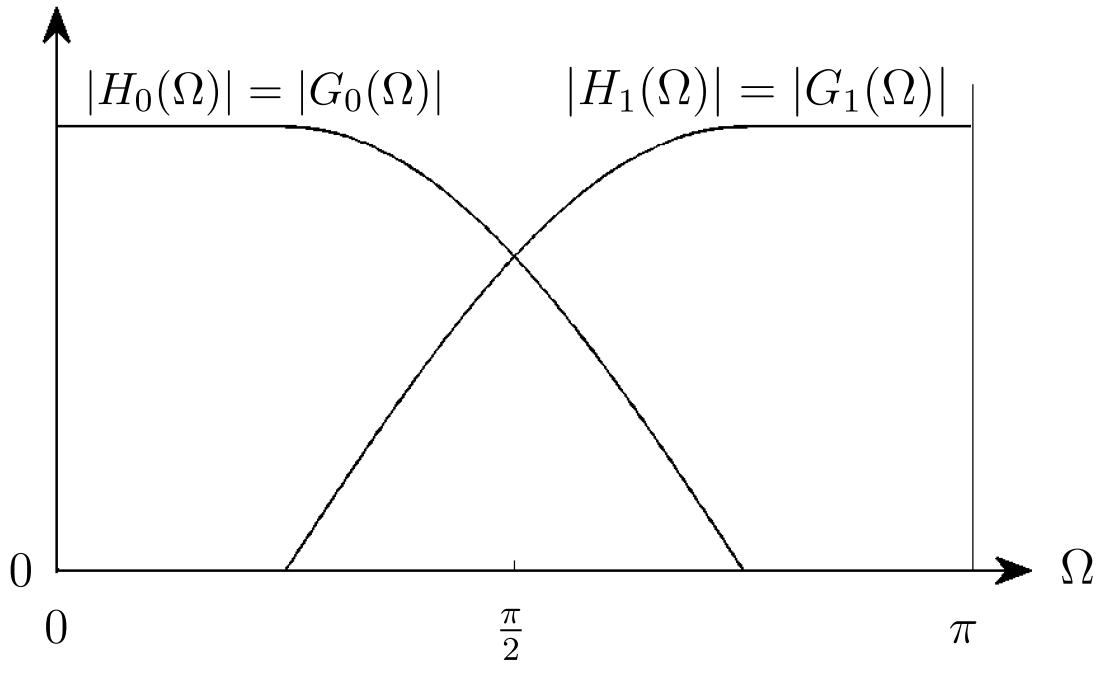
\includegraphics[width=.5\textwidth]{../fig/power_symetric}
\end{center}
Diese Filter werden z.B. in der Speicherung von Sprachsignalen verwendet. 
Dabei werden Signale in einzelne Frequenzbänder zerlegt. Tiefere Frequenzen 
kommen dabei vermehrt vor und können so besser (mehr Bits) quantisiert werden.
\begin{center}
	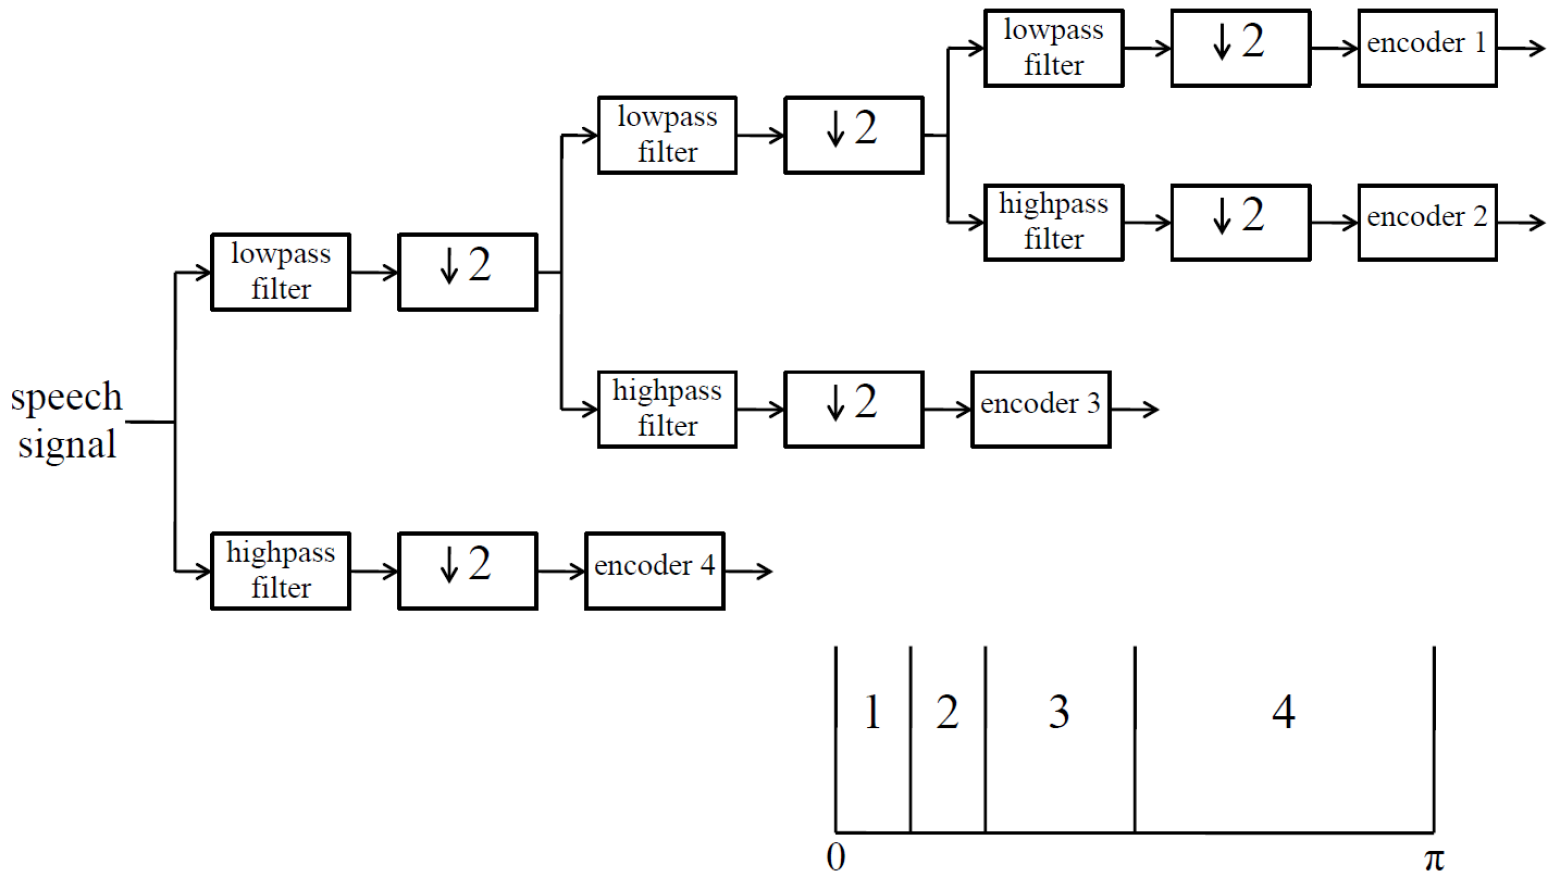
\includegraphics[width=.7\textwidth]{../fig/quadrature_mirror_ex}
\end{center}

%===============================================================================
\section{DFT Filterbank}
Bei dieser Filterbank handelt es sich un eine Generalisierung der Quadratur Spiegel
Filterbank. Die Anzahl Channels wird von $2$ auf $M$ erhöht. Es ergeben sich $M$ 
Filter in der Analyse \& Synthese. Die Subband-Signale können dadurch mit tieferer 
Sampling-Rate abgetastet werden. Es wird unterschieden zwischen:
\begin{itemize}[noitemsep,topsep=3pt]
	\item \textbf{Critical sampling:} Die Anzahl der Filter $H_0(z), H_1(z), \ldots, H_
{M-1}$ entspricht dem Downsampling $M$.
	\item \textbf{Oversampling:} Anzahl Kanäle ist grösser als der Downsampling Faktor.
	\item \textbf{Undersampling:} Anzahl Kanäle ist kleiner als der Downsampling Faktor. 
\end{itemize}
Mit Undersampling ist \emph{keine} perfekte Rekonstruktion des Eingangssignals $x[n]$ 
möglich.
\begin{center}
	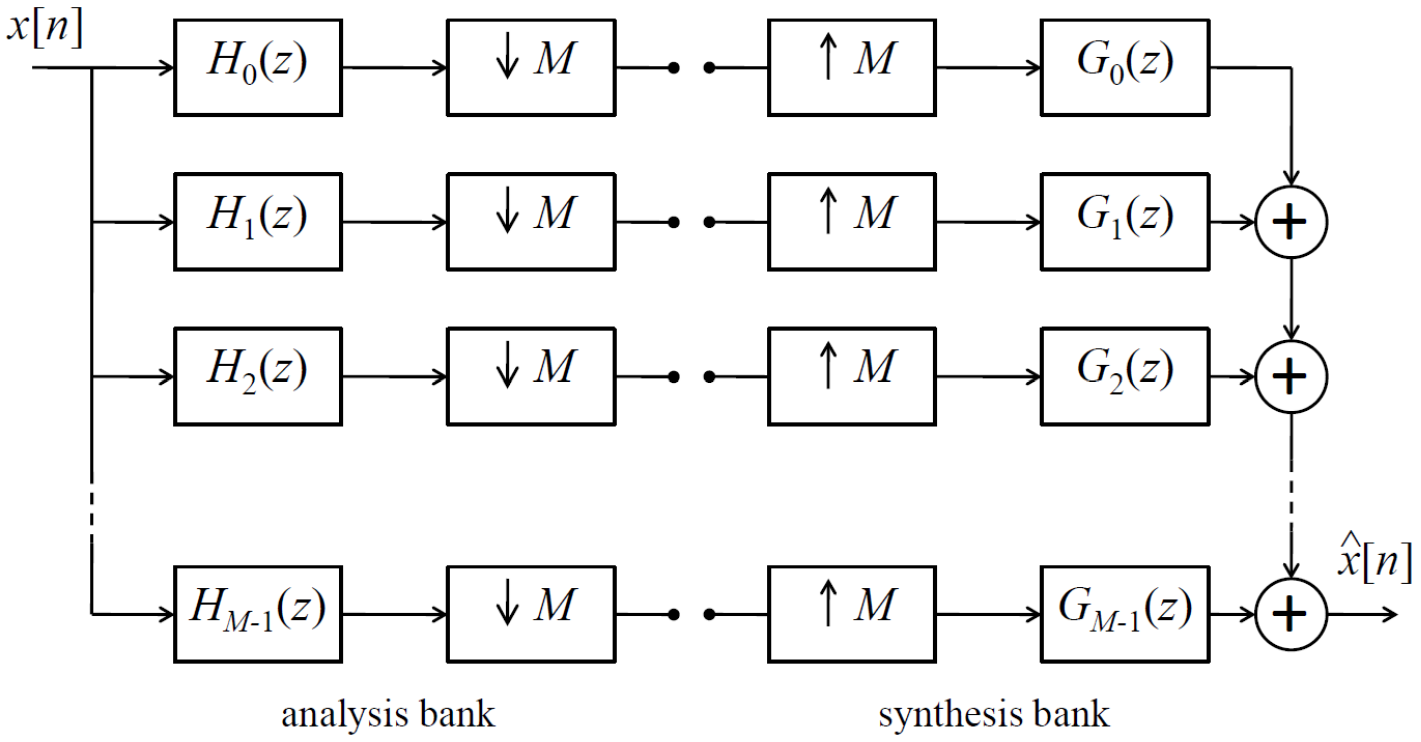
\includegraphics[width=.6\textwidth]{../fig/critical_sampled}
\end{center}
Um ein simpleres Design zu erreichen, wird der Prototype-Filter $H(z)$ (TP) jeweils 
frequenzmässig verschoben. Das selbe gilt für die Synthesis-Bank mit $G(z)$. 
\[ H_l(z) = H(z\cdot\e^{-\im 2\pi l/M}) \qquad l=0,1,\ldots,M-1 \]
\[ G_l(z) = G(z\cdot\e^{-\im 2\pi l/M}) \qquad l=0,1,\ldots,M-1 \]
\begin{center}
	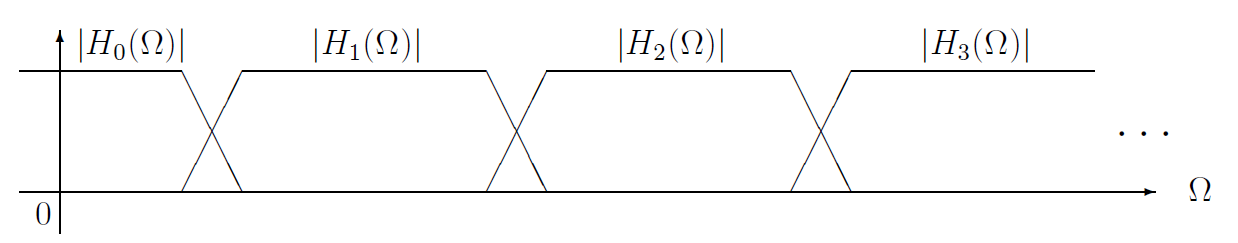
\includegraphics[width=.7\textwidth]{../fig/dft_bank_freq.png}
\end{center}
Frequenzgang:
\[ H_l(\Omega) = H(\Omega-2\pi l/M) \]
Die Namensgebung ist auf die folgende Implementierung zurückzuführen. Das Eingangssignal
wird im $l$-ten Kanal um $2\pi l/M$ geshiftet.
\begin{center}
	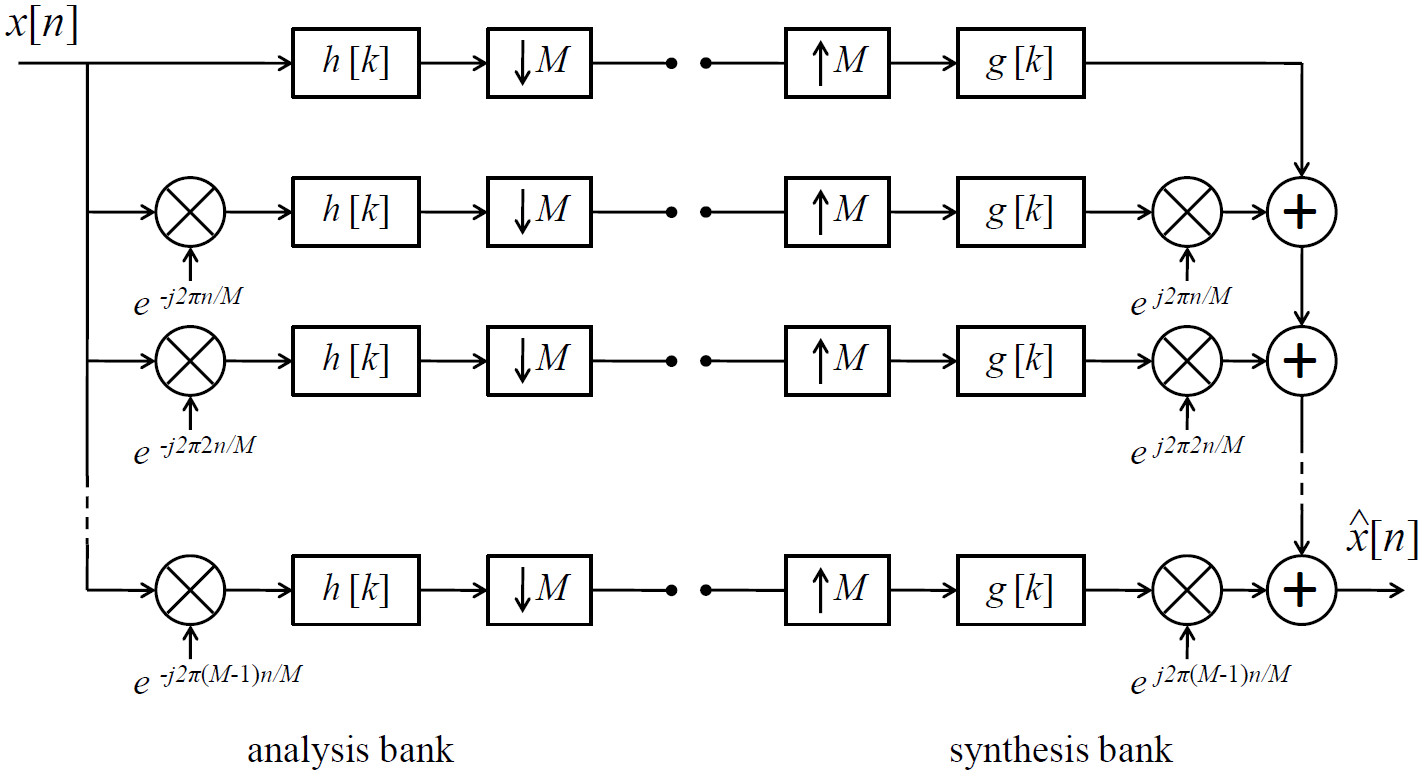
\includegraphics[width=.7\textwidth]{../fig/dft_filterbank_implementation.png}
\end{center}
Die Impulsantworten der Analysis \& Synthesis-Filter lauten:\\
\begin{minipage}{.5\textwidth}
	\[ h[k] = \left\lbrace\begin{matrix}
		1	& \textrm{if } k \in \{0,1,\ldots,M-1\}\\
		0	& \textrm{otherwise}
	\end{matrix}\right. \]
\end{minipage}
\begin{minipage}{.5\textwidth}
	\[ g[k] = \left\lbrace\begin{matrix}
		\frac{1}{M}	& \textrm{if } k \in \{0,1,\ldots,M-1\}\\
		0	& \textrm{otherwise}
	\end{matrix}\right. \]
\end{minipage}
\newpage \noindent

Mit Polyphase kann dies in eine DFT mit Polyphase Filter aufgeteilt werden:
\[ H_l(z) = \sum_{i=0}^{M-1}\e^{\im 2\pi li/M} \cdot (z^{-i} \cdot P_i(z^M) )
	\qquad l=0,1,\ldots,M-1 \]
\begin{minipage}{.6\textwidth}
	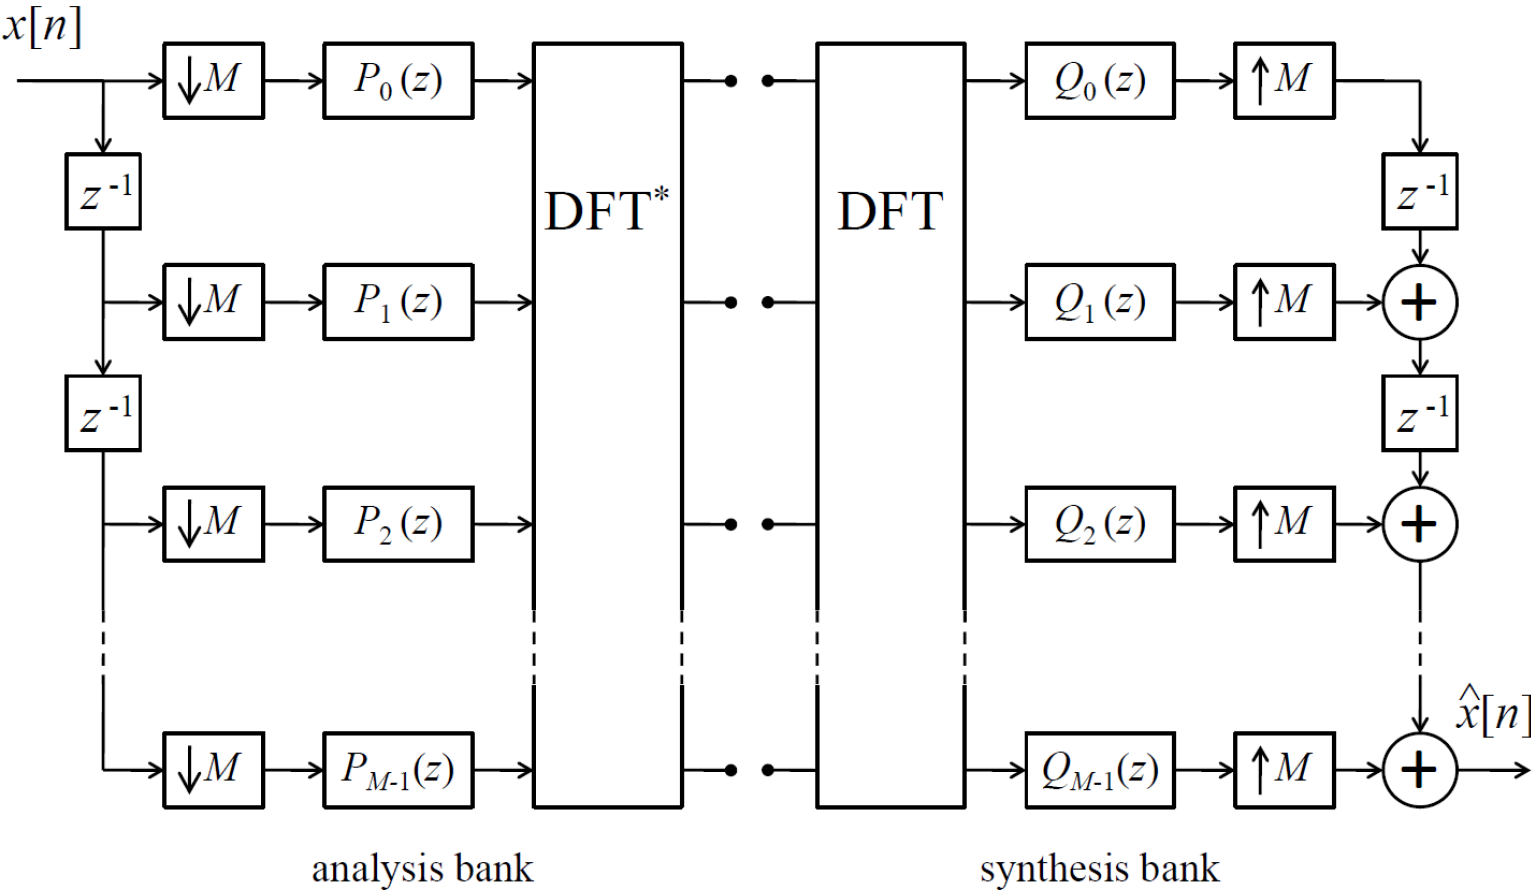
\includegraphics[width=\textwidth]{../fig/dft_filterbank}
\end{minipage}
\begin{minipage}{.4\textwidth}
	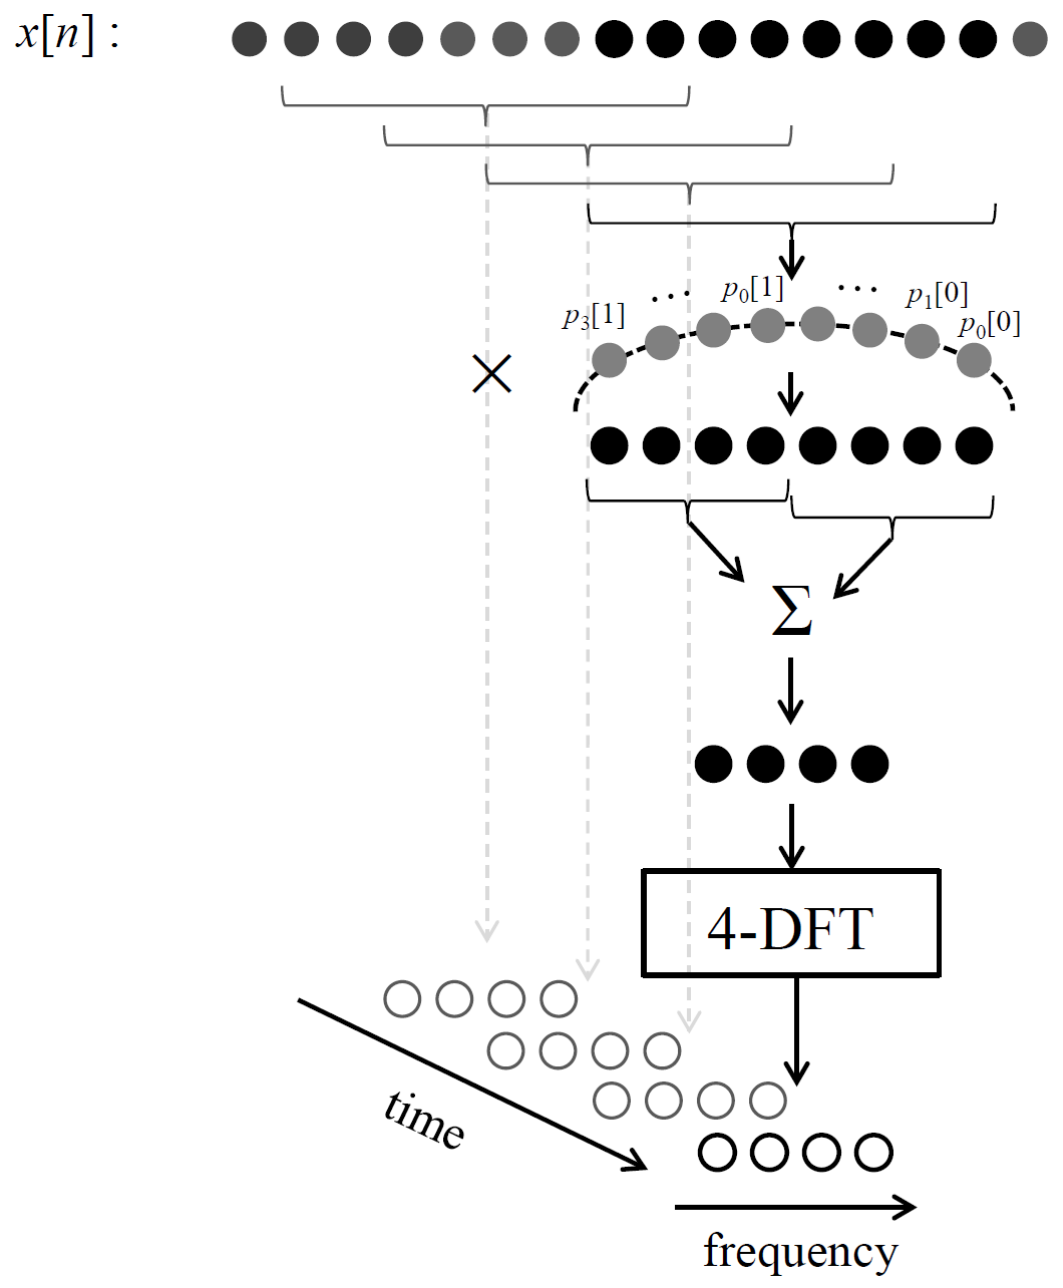
\includegraphics[width=\textwidth]{../fig/dft_filter_ill}
\end{minipage}
Filterbank Ausgangssignal im $z$-Bereich:
\[ \hat{X}(z) = \sum_{i=0}^{M-1}z^{-i} \cdot Q_i(z^M) \cdot \sum_{i=0}^{M-1}Y_l(z^M) \cdot e^{j2\pi li/M} \]
~\\
Vorteile der DFT-Filterbank mit Polyphasen-Struktur:
\begin{itemize}[noitemsep,topsep=3pt]
	\item Es handelt sich um FIR-Filter bei den Polyphase-Komponenten. Dabei handelt es sich um downgesampelte Varianten
	von $h[k]$ und $g[k]$. Diese Filter haben typischerweise einen kleinen Komplexitätsgrad. 
	\item Für die DFT-Berechnungen sind effiziente FFT-Algorithmen verfügbar.
\end{itemize}